\chapter{Introducción específica} % Main chapter title

\label{Chapter2}

%----------------------------------------------------------------------------------------
%	SECTION 1
%----------------------------------------------------------------------------------------
%Todos los capítulos deben comenzar con un breve párrafo introductorio que indique cuál es el contenido que se encontrará al leerlo.  La redacción sobre el contenido de la memoria debe hacerse en presente y todo lo referido al proyecto en pasado, siempre de modo impersonal.
En el presente capítulo se describen los componentes de hardware, software, protocolos de comunicación y plataformas utilizados para realizar el trabajo.

\section{Componentes principales del hardware}
\label{sec:hw:components}

En esta sección se describen los módulos de hardware de terceros utilizados en el trabajo.

\subsection{ESP32-DevKitC}
%https://docs.espressif.com/projects/esp-dev-kits/en/latest/esp32/esp32-devkitc/index.html

La placa ESP32-DevKitC V4, figura \ref{fig:devkit}, es una placa de desarrollo basada en el SoC (\textit{System On Chip}) ESP32 de Espressif Systems. Es una placa popular y versátil ampliamente utilizada por desarrolladores, ingenieros y aficionados para la creación de prototipos y el desarrollo de proyectos de internet de las cosas o IoT (del inglés \textit{Internet of Things}), sistemas embebidos y otras aplicaciones \cite{DEV:KIT}.

Cacterísticas generales:

\begin{itemize}
	%\item Basada en diferentes módulos ESP32.
	\item Microcontrolador con arquitectura de uno o dos núcleos de 32 bits con velocidades de reloj de hasta 240 MHz.
	\item Memoria SRAM integrada.
	%\item Memoria flash integrada para almacenamiento de firmware.
	\item Conectividad Wi-Fi 802.11 b/g/n (2.4 GHz) integrada.
	\item Conectividad bluetooth (classic y low energy) integrada.
	%\item La mayoría de los pines I/O del módulo ESP32 están disponibles a través de pines header para una fácil conexión.
	%\item Permite la conexión de periféricos con cables jumper o el montaje en una placa de pruebas.
	%\item Conector micro USB para alimentación y comunicación.
	%\item Botones de reset y boot integrados para facilitar la programación.
	%\item Compatible con múltiples entornos de desarrollo (ESP-IDF, Arduino IDE, MicroPython).
\end{itemize}

\begin{figure}[h]
\centering
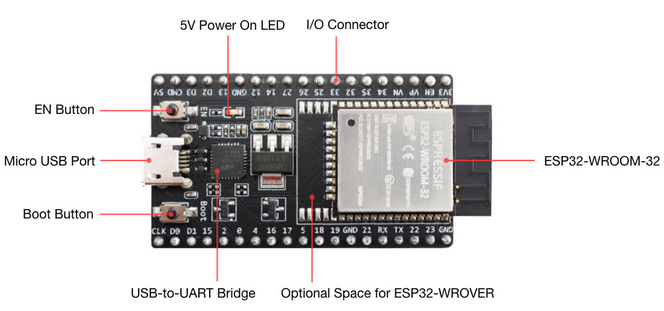
\includegraphics[scale=.5]{./Figures/devkit.png}
	\caption{ESP32-DevKitC V4 con el módulo ESP32-WROOM-32 integrado\protect\footnotemark.}
	\label{fig:devkit}
\end{figure}

\footnotetext{Imagen tomada de \href{https://docs.espressif.com/projects/esp-dev-kits/en/latest/esp32/esp32-devkitc/user_guide.html\#overview}
{https://docs.espressif.com}}



\subsection{Módulo sensor PH-4502C}
El sensor de pH analógico PH-4502C, figura \ref{fig:ph}, es un módulo electrónico diseñado para medir el grado de acidez de soluciones líquidas, típicamente el modelo E201-BNC \cite{PH:4502C}. Este sensor proporciona una salida de tensión analógica que es proporcional al nivel de pH detectado por el electrodo.

Características:

\begin{itemize}
	%\item Módulo electrónico compatible con electrodos de pH con conector BNC.
	\item Rango de detección de pH de 0 a 14.
	\item Salida analógica que varía, entre 0 y 5 VDC, con el pH del liquido.
	%\item Requiere una alimentación de voltaje de 5V DC.
	%\item Corriente de operación entre 5 y 10 mA.
	\item Temperatura de operación del módulo generalmente entre -10 °C y 50 °C.
	%\item Incorpora un potenciómetro para el ajuste del offset o calibración.
	%\item El electrodo tiene un tiempo de estabilización de respuesta de aproximadamente 1 minuto.
\end{itemize}

\begin{figure}[h]
\centering
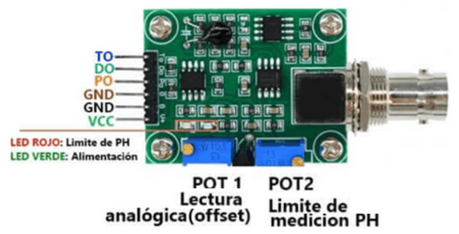
\includegraphics[scale=.5]{./Figures/ph.png}
	\caption{Distribución de pines del módulo PH-4502C\protect\footnotemark.}
	\label{fig:ph}
\end{figure}


\footnotetext{Imagen tomada de \href{https://uelectronics.com/producto/sensor-de-ph-liquido/?srsltid=AfmBOop9186NUUqLe2lmdM_tZTSfz79gsdcGSMFpg6aQvBxj-Fu9oF5t}
{https://uelectronics.com/producto/sensor-de-ph-liquido/}}


%https://uelectronics.com/producto/sensor-de-ph-liquido/?srsltid=AfmBOop9186NUUqLe2lmdM_tZTSfz79gsdcGSMFpg6aQvBxj-Fu9oF5t

\subsection{Módulo medidor de sólidos disueltos totales}

El medidor de sólidos disueltos totales o TDS (del inglés \textit{Total Dissolved Solids}) Meter 1.0, figura \ref{fig:tds}, es un sensor o módulo electrónico diseñado para medir la cantidad total de sustancias orgánicas e inorgánicas disueltas en un líquido, expresada típicamente en partes por millón (ppm) o miligramos por litro (mg/l) \cite{TDS}. Este tipo de sensor se utiliza para evaluar la calidad del agua en diversas aplicaciones como hidroponía, acuicultura, tratamiento de aguas y monitoreo ambiental.

Características:

\begin{itemize}
	%\item Requiere alimentación de 3.3 a 5.5 VDC.
	\item Salida analógica de 0 a 2,3 VDC (proporcional a TDS).
	\item Rango de medición típico de 0 a 1000 ppm.
	%\item Incluye sonda impermeable con electrodos.
	\item Interfaz de 3 pines (VCC, GND, output).
	\item Conector para la sonda (2 pines).
	%\item Compensación de temperatura.
\end{itemize}


\begin{figure}[h]
\centering
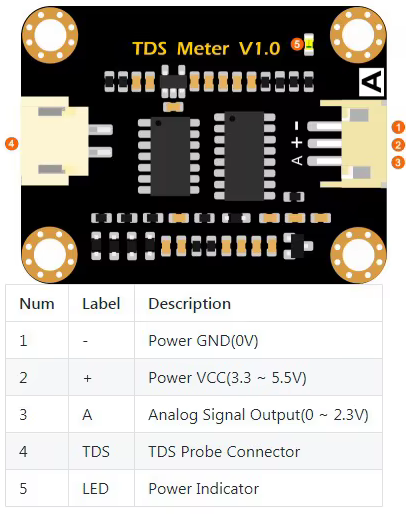
\includegraphics[scale=.5]{./Figures/tds.png}
	\caption{Ilustración del módulo sensor TDS meter v1.0\protect\footnotemark.}
	\label{fig:tds}
\end{figure}

\footnotetext{Imagen tomada de \href{https://www.digikey.be/htmldatasheets/production/2799469/0/0/1/sen0244.html}
{https://www.digikey.be/htmldatasheets}}

\subsection{Sensor de humedad capacitivo V2.0}

El sensor de humedad capacitivo V2.0, figura \ref{fig:moisture}, mide los niveles de humedad mediante detección capacitiva en lugar de resistiva, como otros sensores disponibles. Fabricado con material resistente a la corrosión, ofrece una vida útil prolongada al insertarse en el sustrato alrededor de las plantas \cite{MOISTURE}.

\begin{itemize}
	\item Requiere alimentación de 3,3 a 5,5 VDC.
	\item Corriente de operación de 5 mA.
	\item Salida analógica.
	%\item Incluye un regulador de tensión integrado compatible con MCUs de 3.3V y 5V.
\end{itemize}


\begin{figure}[h]
\centering
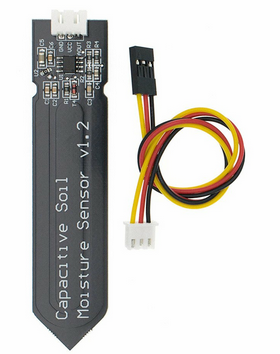
\includegraphics[scale=.5]{./Figures/moisture.png}
	\caption{Módulo sensor de humedad capacitivo\protect\footnotemark.}
	\label{fig:moisture}
\end{figure}

\footnotetext{Imagen tomada de \href{https://probots.co.in/soil-moisture-sensor-capacitive-v1-2.html}
{https://probots.co.in/}}

\subsection{Sensor de temperatura digital DS18B20}

El DS18B20, figura \ref{fig:ds18b20}, es un sensor de temperatura digital que proporciona mediciones en grados Celsius con una resolución configurable de 9 a 12 bits \cite{DS18B20}. %Este sensor se comunica a través de un bus 1-Wire, lo que significa que solo requiere una línea de datos (además de tierra) para la comunicación con un micontrolador. Cada DS18B20 tiene un código de serie único de 64 bits grabado en fábrica, lo que permite que múltiples sensores funcionen en el mismo bus 1-Wire, lo que permite la creación de redes de sensores de temperatura distribuidos.

Características:

\begin{itemize}
	%\item Requiere alimentación de 3.3 a 5.5 VDC.
	\item Rango de medición de temperatura: -55 °C a +125 °C.
	\item Precisión: ±0,5 °C en el rango de -10 °C a +85 °C.
	%\item Resolución configurable: 9, 10, 11 o 12 bits (por defecto 12 bits).
	\item Interfaz de comunicación: 1-Wire (requiere un solo pin digital).
	%\item Cada sensor tiene una dirección única de 64 bits.
	%\item Puede alimentarse a través de la línea de datos (\textit{parasite power}) o con una fuente externa.
	%\item Tiempo de conversión de temperatura: hasta 750 ms (para resolución de 12 bits).
	%\item Disponible en encapsulado TO-92 y en versiones con sonda impermeable.
\end{itemize}


\begin{figure}[h]
\centering
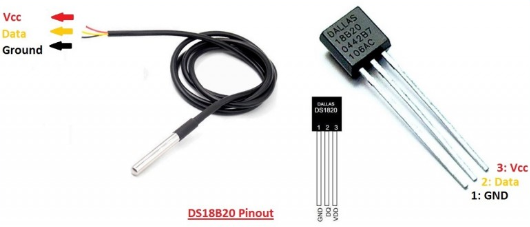
\includegraphics[scale=.5]{./Figures/ds18b20.png}
	\caption{Pinout del sensor DS18B20 y presentación del chip con su vaina protectora característica\protect\footnotemark.}
	\label{fig:ds18b20}
\end{figure}


\footnotetext{Imagen tomada de \href{https://tienda.ityt.com.ar/sensor-temp-hum-ic/1694-sensor-temperatura-ds18b20-18b20-1-wire-one-wire-itytarg.html}
{https://tienda.ityt.com.ar/sensor-temp-hum-ic/}}

%https://tienda.ityt.com.ar/sensor-temp-hum-ic/1694-sensor-temperatura-ds18b20-18b20-1-wire-one-wire-itytarg.html

\subsection{Sensor de luz ambiental digital BH1750}

El circuito integrado BH1750, figura \ref{fig:BH1750}, es un sensor de luz ambiental digital con interfaz de bus I2C (\textit{Inter-Integrated Circuit}) \cite{BH1750}. Este sensor es capaz de detectar un amplio rango de intensidad luminosa, desde 1 hasta 65535 lux, con una resolución de 16 bits. El chip proporciona una salida digital directa, lo que elimina la necesidad de cálculos complejos.

%Características:

%\begin{itemize}
	%\item Requiere alimentación de 3.3 a 5.5 VDC.
	%\item Interfaz de comunicación I2C.
	%\item Rango de medición de 1 a 65535 lux.
	%\item Resolución: 16 bits.
%\end{itemize}

\begin{figure}[h]
\centering
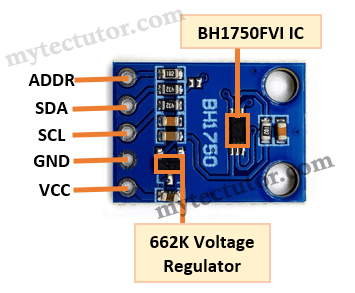
\includegraphics[scale=.5]{./Figures/BH1750.png}
	\caption{Pinout del módulo de adaptación del sensor BH1750\protect\footnotemark.}
	\label{fig:BH1750}
\end{figure}


\footnotetext{Imagen tomada de \href{https://mytectutor.com/bh1750-ambient-light-sensor-with-arduino/}
{https://mytectutor.com/}}

%https://mytectutor.com/bh1750-ambient-light-sensor-with-arduino/


\section{Componentes principales del software}
\label{sec:sw:components}
En esta sección se describen las herramientas de software de terceros utilizados en el trabajo.


\subsection{ESP-IDF}

ESP-IDF (\textit{Espressif IoT Development Framework}) es un conjunto de herramientas de desarrollo integral provisto por Espressif Systems. Este framework facilita la creación de firmware para su línea de SoCs ESP32 y ESP8266. Incluye un sistema operativo en tiempo real (FreeRTOS), bibliotecas con APIs para diversos periféricos y protocolos (Wi-Fi, bluetooth, TCP/IP), compilador (basado en GCC), depurador (GDB) y utilidades para la construcción, flasheo y monitoreo de proyectos. ESP-IDF permite a los desarrolladores escribir aplicaciones en C o C++, quienes aprovechan así la potencia y la conectividad de los chips de Espressif \cite{ESPIDF}.


\subsection{FreeRTOS}

FreeRTOS es un sistema operativo en tiempo real (RTOS) popular y de código abierto. Ofrece un núcleo pequeño y eficiente, apropiado para microcontroladores y sistemas con recursos limitados. Proporciona mecanismos de multitarea, como hilos (tareas), gestión de memoria, sincronización y comunicación entre tareas (semáforos, mutexes, colas). Facilita la organización y la gestión de la ejecución de múltiples funciones de manera concurrente y determinista, crucial para aplicaciones de tiempo real. Su portabilidad permite su uso en una amplia variedad de arquitecturas de procesadores \cite{FREERTOS}.

\subsection{Ceedling}

Ceedling es un framework de construcción y prueba para proyectos de software embebido en C. Automatiza tareas como la compilación, el enlazado y la ejecución de pruebas unitarias. Integra herramientas como Unity, CMock y Ruby. Facilita la adopción de prácticas de desarrollo basadas en pruebas (TDD) y asegura la calidad del código mediante la verificación automatizada de unidades de software individuales \cite{CEEDLING}.

\subsection{React Native}
React Native es un framework de código abierto desarrollado por Meta. Permite la creación de aplicaciones móviles para plataformas iOS y Android desde una única base de código JavaScript. Utiliza los mismos bloques de construcción de la interfaz de usuario que las aplicaciones nativas. Esto resulta en aplicaciones con apariencia y rendimiento nativos \cite{reactnative}.

\section{Protocolos de comunicación empleados}

A continuación, se detallan los protocolos de comunicación empleados en la realización del trabajo.

\subsection{HTTP}
HTTP (\textit{Hypertext Transfer Protocol}) es un protocolo de aplicación que define cómo los clientes (navegadores web) solicitan recursos (páginas web, imágenes, etc.) a los servidores y cómo estos responden. Utiliza un modelo de petición-respuesta. Las peticiones HTTP incluyen un método (GET, POST, PUT, DELETE, etc.) que indica la acción que el cliente desea realizar. Las respuestas HTTP contienen un código de estado que informa sobre el resultado de la petición \cite{HTTP}.

\subsection{I2C}
I2C es un protocolo de comunicación serial síncrono, multi-maestro/esclavo, de baja velocidad y corta distancia. Utiliza solo dos líneas bidireccionales: SDA (datos seriales) y SCL (reloj serial), ambas conectadas a través de resistencias \textit{pull-up}. Permite que múltiples dispositivos se comuniquen entre sí en el mismo bus. Los maestros inician la comunicación y controlan el reloj, mientras que los esclavos responden a las peticiones de los maestros \cite{I2C}.

\subsection{1-Wire}
1-Wire es un protocolo de comunicación serial semidúplex. Utiliza un único conductor para la comunicación de datos y, en algunos casos, para la alimentación. Un maestro controla la comunicación con uno o varios dispositivos esclavos en el mismo bus. El protocolo es relativamente lento pero resulta económico para conectar sensores, memorias y otros dispositivos de baja velocidad, especialmente en aplicaciones donde el bajo número de pines es limitado \cite{1WIRE}.










